\documentclass{beamer}    % 14pt je nenujen
\usepackage[T1]{fontenc}
\usepackage[utf8]{inputenc}
\usepackage[slovene]{babel}
\usepackage{pgfpages}           % privat zapiski
\usepackage{amsfonts}
\usepackage{amsmath,amsthm}     % pravilen izpis v "math mode"
%\usepackage{hyperref}
\usepackage{graphicx}           % za slike
\usepackage{tikz}
\usepackage{multicol}
\usepackage{ulem}
\usepackage{bibentry}

%\hypersetup{hidelinks}

\setbeamertemplate{theorems}[ams style]             % numbered da brez bold 

\setbeameroption{hide notes}                        % samo prosojnice
%\setbeameroption{show only notes}                   % samo zapiski
%\setbeameroption{show notes on second screen=right}  % oboje

\usepackage{palatino}
\usefonttheme{serif}

%\usecolortheme{beetle} %ali beetle morda ali seagull 

\setbeamertemplate{navigation symbols}{} % izklop navigacije
\setbeamertemplate{footline}[frame number]{} % oštevilčenje
\setbeamertemplate{note page}{\pagecolor{yellow!5}\insertnote}

\newtheorem{izrek}{Izrek}
\newtheorem{trditev}[izrek]{Trditev}
\newtheorem{posledica}[izrek]{Posledica}
\newtheorem{definicija}[izrek]{Definicija}
\newtheorem{naloga}[izrek]{Naloga}
\newtheorem{resitev}[izrek]{Naloga}

\author{Tim Kalan \\ \medskip
        \footnotesize Mentor: izred.~prof.~dr. Marjetka Knez}
\institute[FMF]{Fakulteta za matematiko in fiziko}
\title{
    Spodbujevano učenje pri igranju namiznih iger \\ 
    \large (angl. \textit{Reinforcement learning in board games})}
\date{20. november 2020} 



\begin{document}

\begin{frame}
    \titlepage
\end{frame}


\begin{frame}
    \frametitle{Strojno učenje}
    \begin{itemize}
        \item Nadzorovano učenje \textit{(npr. prepoznavanje števk)}
        \item Nenadzorovano učenje \textit{(npr. razvrščanje)}
        \item \textbf{Spodbujevano učenje}
    \end{itemize}
\end{frame}


\begin{frame}
    \frametitle{Motivacija: Instrumentalno pogojevanje}
    \begin{itemize}
        %http://www.edugyan.in/2017/03/edward-lee-thorndike-theory-of-learning.html, 
        %https://en.wikipedia.org/wiki/Reinforcement
        \item Lepa psihološko motivirana podlaga
        \item \textbf{Nagrade in kazni} 
    \end{itemize}

    \begin{figure}[b]
        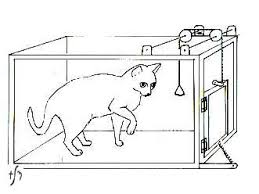
\includegraphics[scale=0.47]{slike/macka.jpg}
        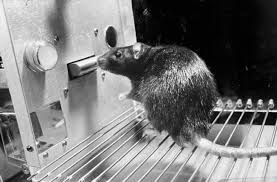
\includegraphics[scale=0.5]{slike/miska.jpg}
    \end{figure}
\end{frame}


\begin{frame}
    \frametitle{Motivacija: Zakaj namizne igre?}
    \begin{itemize}
        \item Aplikacija abstraktnega mišljenja.
        \item Spremljajo človeštvo že zelo dolgo.
        \item ">Modelirajo"< resnično življenje.
        \item Uporabno mesto za testiranje algoritmov.
    \end{itemize}
\end{frame}


\begin{frame}
    \frametitle{Spodbujevano učenje - osnovni koncepti 1}
    \begin{multicols}{2}
    \begin{itemize}
        \item Nagrada
        \item Agent
        \item Okolje
        \item Stanje
        \item Akcija
        %https://sl.wikipedia.org/wiki/Spodbujevano_učenje
    \end{itemize}
    \end{multicols}

    \begin{figure}
        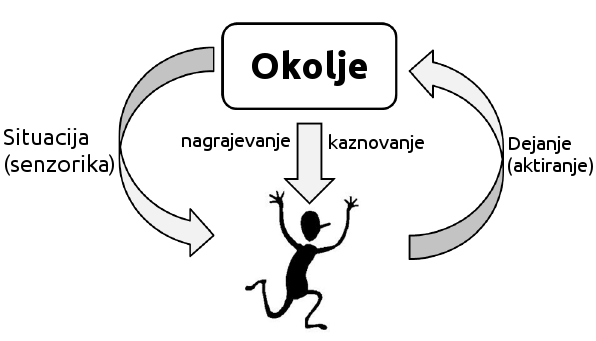
\includegraphics[scale=0.5]{slike/RLloop.png}
    \end{figure}
\end{frame}


\begin{frame}
    \frametitle{Spodbujevano učenje - osnovni koncepti 2}
    \begin{itemize}
        \item Pomemben je čas.
        \item Ne poznamo ">pravilnih"< akcij.
        \item Raziskovanje in izkoriščanje
    \end{itemize}
\end{frame}


\begin{frame}
    \frametitle{RL agent}
    \begin{itemize}
        \item Strategija (angl. \textit{Policy})
        \item Vrednostna funkcija (angl. \textit{Value function})
        \item (Model)
    \end{itemize}
\end{frame}


\begin{frame}
    \frametitle{Kje je to uporabno?}
    \begin{itemize}
        \item Naučiti robota hoje.
        \item Upravljati s portfeljem.
        \item Igrati namizne igre.
        \item Igrati katerekoli igre.
        \item ...
    \end{itemize}
    \medskip
    \emph{Praktično karkoli, kjer lahko cilj modeliramo kot numerične
    nagrade, ne poznamo pa optimalnih akcij za dostop do teh nagrad.}
\end{frame}


\begin{frame}
    \frametitle{Problem}
    \begin{definicija}[Hipoteza o nagradi]
        Vse cilje je mogoče opisati kot maksimizacijo neke kumulativne numerične 
        nagrade.
    \end{definicija}

    \medskip

    \begin{itemize}
        \item Je to vedno res?
    \end{itemize}
\end{frame}


\begin{frame}
    \frametitle{Primer: Križci in krožci 1}
    \tikzstyle{block} = [rectangle, draw, 
    text width=5em, text centered, rounded corners, minimum height=4em]
    \tikzstyle{line} = [draw, -latex]
    \begin{tikzpicture}[node distance = 6em, auto, thick]
        \node [block] (Agent) {Agent};
        \node [block, below of=Agent] (Okolje) {Okolje};
        \path [line] (Agent.0) --++ (4em,0em) |- node [near start]{Akcija $A_t$} (Okolje.0);
        \path [line] (Okolje.190) --++ (-5em,0em) |- node [near start] {Novo stanje  $S_{t+1}$} (Agent.170);
        \path [line] (Okolje.170) --++ (-4.25em,0em) |- node [near start, right] {Nagrada $R_{t+1}$} (Agent.190);
    \end{tikzpicture}
    \begin{itemize}
        \item \textbf{Stanje:} Kje je prazno, kje ">X"< in kje ">O"<.
        \item \textbf{Agent:} Program, ki se odloča, kako igrati.
        \item \textbf{Okolje:} Agentu sporoča nagrade in stanje.
        \item \textbf{Nagrada:} Pozitivna za zmago, negativna za poraz.
        \item \textbf{Akcija:} Postavitev ">X"< oz. ">O"< na ploščo.
    \end{itemize}
\end{frame}


\begin{frame}
    \frametitle{Primer: Križci in krožci 2}
    \begin{itemize}
        \item Agent igra igre, posodablja svoje vrednosti stanj glede na odgovor okolja.
        \item Kako naj to stori?
    \end{itemize}
\end{frame}


\begin{frame}
    \frametitle{Primer: Križci in krožci 3}
    \begin{itemize}
        \item Enostavna ideja:                                  
        %
        $$
        V(s) \leftarrow V(s) + \alpha [V(s') - V(s)]
        $$
        %                                       
        \pause
        \item $s$ je trenutno stanje                     
        \pause
        \item $V$ je vrednostna funkcija                 
        \pause
        \item $\alpha$ je velikost koraka (hitrost učenja) 
        %\pause
        %\item $R$ je nagrada   
        %\pause
        %\item $\gamma$ je diskontni faktor (pomemben je čas)    
        \pause
        \item $s'$ je stanje, ki sledi \textit{s}   
    \end{itemize}
    \medskip
    \emph{Zgornje je primer \textbf{učenja s časovno razliko}} (angl. \textit{Temporal difference learning})
\end{frame}


\begin{frame}
    \frametitle{Bistvo}
    %
    $$
    \textit{nova ocena} \leftarrow \textit{stara ocena} + \textit{korak} 
    [\textit{tarča} - \textit{stara ocena}]
    $$
    %
    \medskip
    \begin{itemize}
        \item Tako ocenimo dano strategijo.
        \item Kako pa strategijo dejansko spremenimo?
    \end{itemize}
\end{frame}


\begin{frame}
    \frametitle{$\epsilon$-požrešna izboljšava strategije}
    \only<1>{Izberemo ">najboljšo"< akcijo.}
    \pause
    \sout{Izberemo ">najboljšo"< akcijo.}
    \pause
    \medskip

    \begin{itemize}
        \item ">Ponavadi"< izberemo ">najboljšo"< akcijo.
        \item Z verjetnostjo $\epsilon$ izberemo naključno akcijo.
    \end{itemize}

    \begin{figure}
        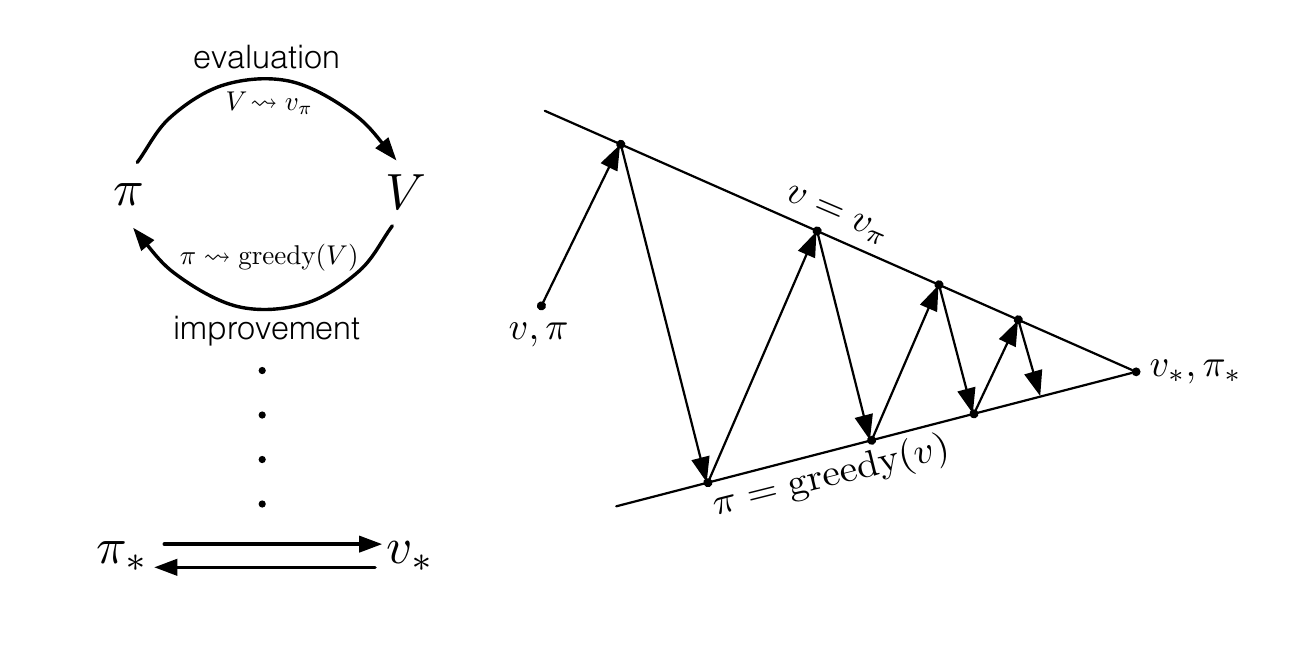
\includegraphics[scale=0.23]{slike/policy-iteration.png}
    \end{figure}
\end{frame}


\begin{frame}
    \frametitle{Alternativa: Monte Carlo spodbujevano učenje 1}
    \begin{definicija}
        \begin{itemize}
            \item Agentova \textbf{strategija} je takšna preslikava $\pi: S \rightarrow A$
                    da velja 
                    \begin{align*}
                    a &= \pi(s) \\
                    \pi(a | s) &= P(A_t = a | S_t = s). 
                    \end{align*}

            \item Naj bodo $R_{t+1}, ...,R_T$ nagrade, ji jih bomo prejeli od trenutka 
                    $t$ do konca epizode. \textbf{Povračilo} $G_t$ definiramo kot
                    $$
                    G_t = R_{t+1} + \gamma R_{t+2} + ... + \gamma^{T-1} R_T.
                    $$

            \item Naj bo $\pi$ dana strategija agenta. \textbf{Vrednostna funkcija 
                    stanja} glede na dano strategijo $v_\pi(s)$ je
                    $$
                    v_\pi(s) = \mathbb{E} [G_t | S_t = s].
                    $$
        \end{itemize}
    \end{definicija}
\end{frame}


\begin{frame}
    \frametitle{Alternativa: Monte Carlo spodbujevano učenje 2}
    \begin{itemize}
        \item Ob obisku stanja $s$: 
        \begin{align*}
            N(s) &\leftarrow N(s) + 1 \\
            S(s) &\leftarrow S(s) + G_t
        \end{align*}
        \item Po koncu učenja: 
        $$
        V(s) \leftarrow S(s) / N(s)
        $$
       \item Pomni: Računanje povprečja zaporedja $(X_i)_{i \in \mathbb{N}}$
       $$
       \mu_k = \frac{1}{k} \sum_{j=1}^k X_j = \mu_{k-1} + \frac{1}{k} (X_k - \mu_{k-1})
       $$
       \item Inkrementalni Monte Carlo:
       $$
       V(s) \leftarrow V(s) + \alpha (G_t - V(S_t))
       $$
    \end{itemize}
\end{frame}


%\begin{frame}
%    \frametitle{Formalizacija: Markovski proces odločanja 1}
%    \begin{definicija}[Markovska veriga]
%        Skučajni proces $(S_t)_{t=0}^T$ na končnem verjetnostnem prostoru 
%        $(\Omega, P)$ je \textbf{Markovska veriga}, če velja Markovska lastnost
%        $$
%        P(S_{t+1} = s_{t+1} | S_{t} = s_{t}, ..., S_0 = s_0) = P(S_{t+1} = s_{t+1} | S_{t} = s_{t})
%        $$
%    \end{definicija}
%    \pause
%    \medskip
%    \begin{itemize}
%        \item Prihodnost je neodvisna od preteklosti, če poznamo sedanjost
%        \pause
%        \item $p_{ss'} := P(S_{t+1} = s' | S_{t} = s) \rightarrow
%                \mathcal{P} := [p_{ss'}]_{s,s'\in \mathcal{S} }$, $\mathcal{S}$ 
%                je množica stanj
%        \item \emph{Markovska veriga} je torej dvojica $(\mathcal{S}, \mathcal{P})$
%    \end{itemize}
%    
%\end{frame}
%
%
%\begin{frame}
%    \frametitle{Formalizacija: Markovski proces odločanja 2}
%    %\begin{definicija}[Markovski proces]
%    %    \textbf{Markovski proces} je par $(\mathcal{S}, \mathcal{P})$, kjer je
%    %    \begin{itemize}
%    %        \item $\mathcal{S}$ je (končna) množica stanj
%    %        \item $\mathcal{P}$ je prehodna matrika
%    %    \end{itemize}
%    %\end{definicija}
%    %\pause
%    \begin{definicija}[Markovski proces odločanja]
%        \textbf{Markovski proces odločanja} je nabor 
%        $(\mathcal{S}, \mathcal{A}, \mathcal{P}, \mathcal{R}, \gamma)$, kjer je
%        \begin{itemize}
%            \item $\mathcal{S}$ je (končna) množica stanj
%            \item $\mathcal{A}$ je (končna) množiza akcij oz. dejanj
%            \item $\mathcal{P}$ je prehodna matrika, kjer $p_{ss'}^a = P(S_{t+1} = s' | S_{t} = s, A_t = a)$
%            \item $\mathcal{R}$ je nagradna funkcija $\mathcal{R}_s^a = E[R_{t+1} | S_{t} = s, A_t = a]$
%            \item $\gamma \in [0, 1]$ je diskontni faktor
%        \end{itemize}
%    \end{definicija}
%\end{frame}


\begin{frame}
    \frametitle{Kam gremo od tu?}
    \begin{itemize}
        \item Koliko stanj imamo?
        \item Do kje lahko pridemo?
        \item Kaj je rešitev?
        \medskip 
        \medskip
        \medskip
        \item Monte Carlo metode ponavadi nastopijo, ko nekaj aproksimiramo, 
                kako je s tem v našem primeru?
    \end{itemize}
\end{frame}


\begin{frame}
    \frametitle{Ideje za naprej}
    \begin{itemize}
        \item Drugi algoritmi
        \item Problem časovne dodelitve zaslug
        \item Večje igre - nevronske mreže
        \item Različni tipi učenja 
    \end{itemize}
\end{frame}


\begin{frame}
    \frametitle{Literatura}
    \begin{thebibliography}{9}
        \bibitem{RLintro} 
        Richard S. Sutton and Andrew G. Barto. 
    \textit{Reinforcement Learning: An introduction}.
    The MIT Press, 
    2015.

    \medskip
    \medskip

    \bibitem{RLboard}
    Imran Ghory.
    \textit{Reinforcement learning in board games}.
    2004.

    \end{thebibliography}
\end{frame}


\end{document}
